\documentclass{article}

\usepackage{shyne}

% document format
\topmargin 0in
\oddsidemargin 0in
\evensidemargin 0in
\headheight 0in
\headsep 0in
\topskip 0in
\textheight 9in
\textwidth 6.5in
\linespread{1.3}


\begin{document}

\begin{flushleft}
\section*{Group Work - Week 4}
\paragraph{1} The maximum monthly fine particulate matter pollution in Minnesota from 2007 to 2009 is below. The data can be found on D2L as ``max\_air\_pol.csv". Use classes 10-15, 15-20, 20-25, etc. 

\[  25.82 ,\,  28.87 ,\, 36.18 ,\, 21.22 ,\, 25.94 ,\, 25.10 ,\, 24.49 ,\, 36.94 ,\, 23.20 ,\, 25.72 ,\, 27.94 ,\, 43.34 \] 
\[31.46 ,\, 38.32 ,\, 24.82 ,\, 22.78 ,\, 28.48 ,\, 24.27 ,\, 24.26 ,\, 15.52 ,\, 22.88 ,\, 15.95 ,\, 14.48 ,\, 23.83 \]
\[ 28.72 ,\, 25.87 ,\, 22.38 ,\, 21.21 ,\, 19.90 ,\, 32.25 ,\, 24.69 ,\, 23.14 ,\, 23.81 ,\, 17.05 ,\, 24.09 ,\, 49.88 \]
\begin{itemize}
\item [(a)] Build a frequency table of the data. Does the data appear to have a normal distribution? Add relative frequency and cumulative frequency tables.//
\bigskip
\bt{The distribution does not seem to be normal. The distribution is not symmetric There do not appear to be any outliers.}\\
\bigskip

{\centering
\begin{table}[ht]
\centering
\begin{tabular}{rrr}
\hline
& Frequency & Cumulative \\
\hline
(10,15] &
1 &
1 \\
(15,20] &
4 &
5 \\
(20,25] & 15 & 20 \\
(25,30] &
9 & 29 \\
(30,35] &
2 & 31 \\
(35,40] &
3 & 34 \\
(40,45] &
1 & 35 \\
(45,50] &
1 & 36 \\
\hline
\end{tabular}
\end{table}\par}


\vspace{.5in}
\item[(b)] Sketch a histogram of the data. Does the histogram show a normal distribution? If not, which characteristic of normal distributions does it violate?\\
\bigskip
\bt{The histogram does not appear to be normal. It is not symmetric. It is skewed to the right.}
\bigskip

{\centering
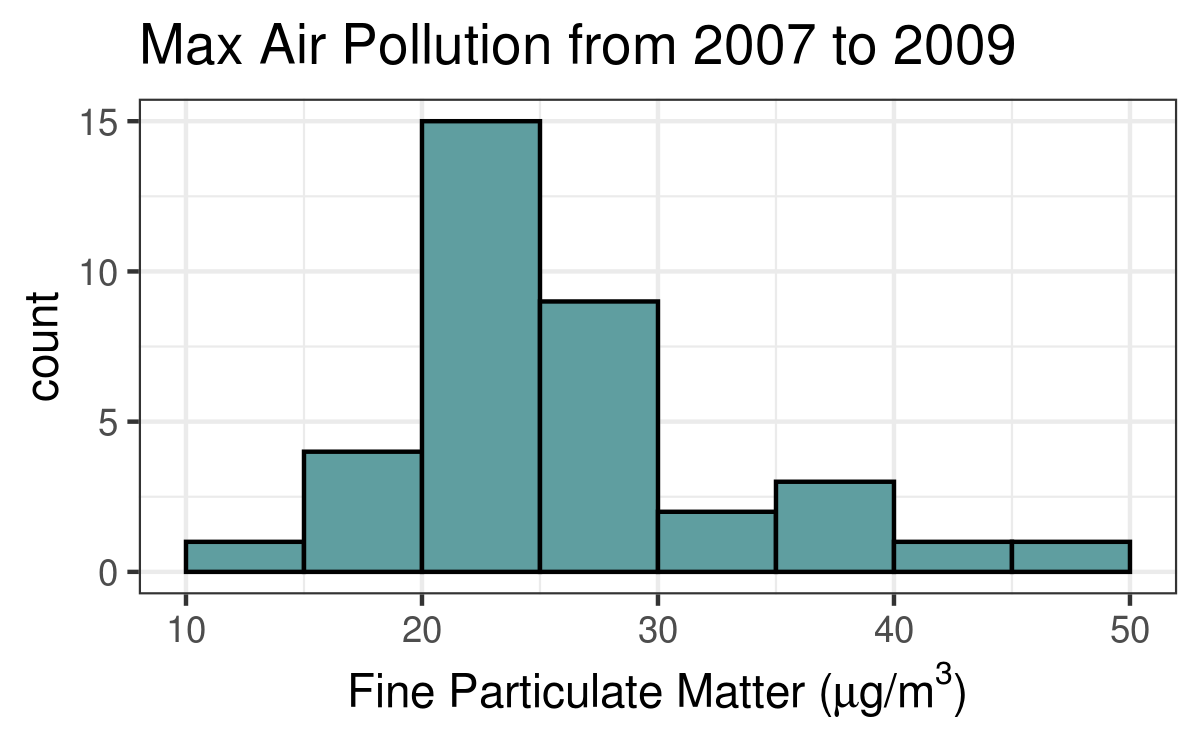
\includegraphics[width=4in]{images/group04_Q2_b}
\par}

\end{itemize}


\newpage
\paragraph{2} The file ``max\_temp\_dec17.csv" on D2L contains the daily high temperatures (in F) for December. 
\begin{itemize}
\item [(a)] Find the mean, median, mode and midrange of the sample. What is the most appropriate measure of center for this data?\\

\bigskip
{\centering
\begin{tabular}{cccc}
Mean & Median & Mode & Midrange \\ 
  \hline
24.65 &  25 & 22, 24, 29 & 24.50 \\ 
\end{tabular}
\par}
\bigskip
\bt{Since temperatures are roughly normal and symmetric, mean is the most appropriate measure of center.}
\vspace{.5in}



\item[(b)] Find the range, variance and standard deviation of the sample. Be sure to include the correct units for each measure.\\

\bigskip
{\centering
\begin{tabular}{ccc}
 Range & Variance & SD \\ 
  \hline
 65 \textdegree F & 252.90 (\textdegree F)$^2$ & 15.90 \textdegree F \\ 
\end{tabular}
\par}

\vspace{.5in}
\end{itemize}


\newpage
\paragraph{3} The file ``mpls\_home\_sales.csv" on D2L contains the adjusted sale prices (in dollars) of a sample of home sold in Minneapolis in 2016. 
\begin{itemize}
\item [(a)] Find the mean, median, mode and midrange of the sample. What is the most appropriate measure of center for this data?\\

\bigskip
{\centering
\begin{tabular}{cccc}
Mean & Median & Mode & Midrange \\ 
  \hline
234980.59 & 202750.00 & 175000 & 451000.00 \\ 
\end{tabular}
\par}
\bigskip
\bt{By looking at the histogram, we can see that the data is right skewed with a few extremely high values. Thus, median is the most appropriate measure of center.}

\bigskip
{\centering
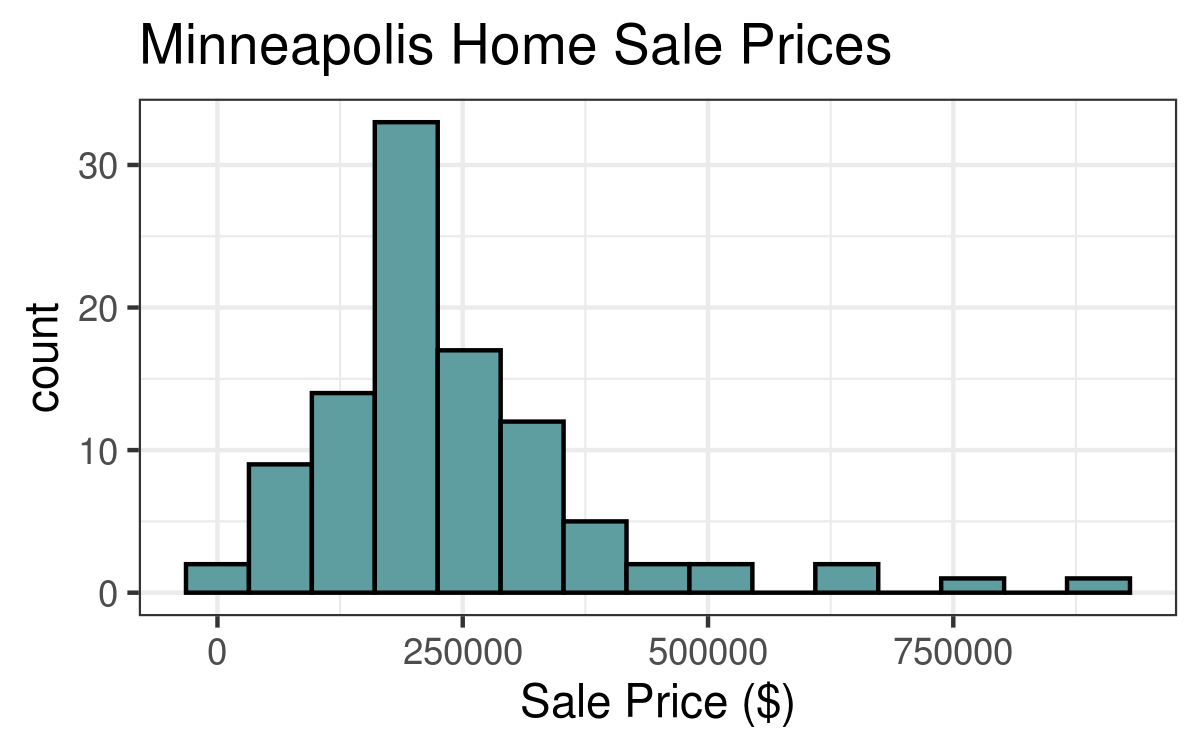
\includegraphics[width=4in]{images/group04_Q2_a}
\par}

\vspace{.5in}


\item[(b)] Find the range, variance and standard deviation of the sample. Be sure to include the correct units for each measure.\\

\bigskip
{\centering
\begin{tabular}{ccc}
Range & Variance & SD \\ 
  \hline
898000 \$ & 21434941764.24 \$$^2$ & 146406.77 \$ \\ 
\end{tabular}
\par}
\vspace{.5in}

\end{itemize}


\newpage
\paragraph{4} For each scenario below, identify some of the graphs that would be appropriate for this data. Create one appropriate graph and use it to answer the research question.

\begin{itemize}
\item [(a)] The data set ``faithful.csv" contains a sample of eruptions of the Old Faithful geyser in Yellowstone National Park. Length of eruption (in minutes) and waiting time until the next eruption (in minutes) are recorded. Researchers want to know if the is a relationship between eruption lengths and waiting times.\\
\bigskip
\bt{Because the question concerns the relationship between two quantitative variables, a scatterplot is most appropriate. }
\bigskip

{\centering
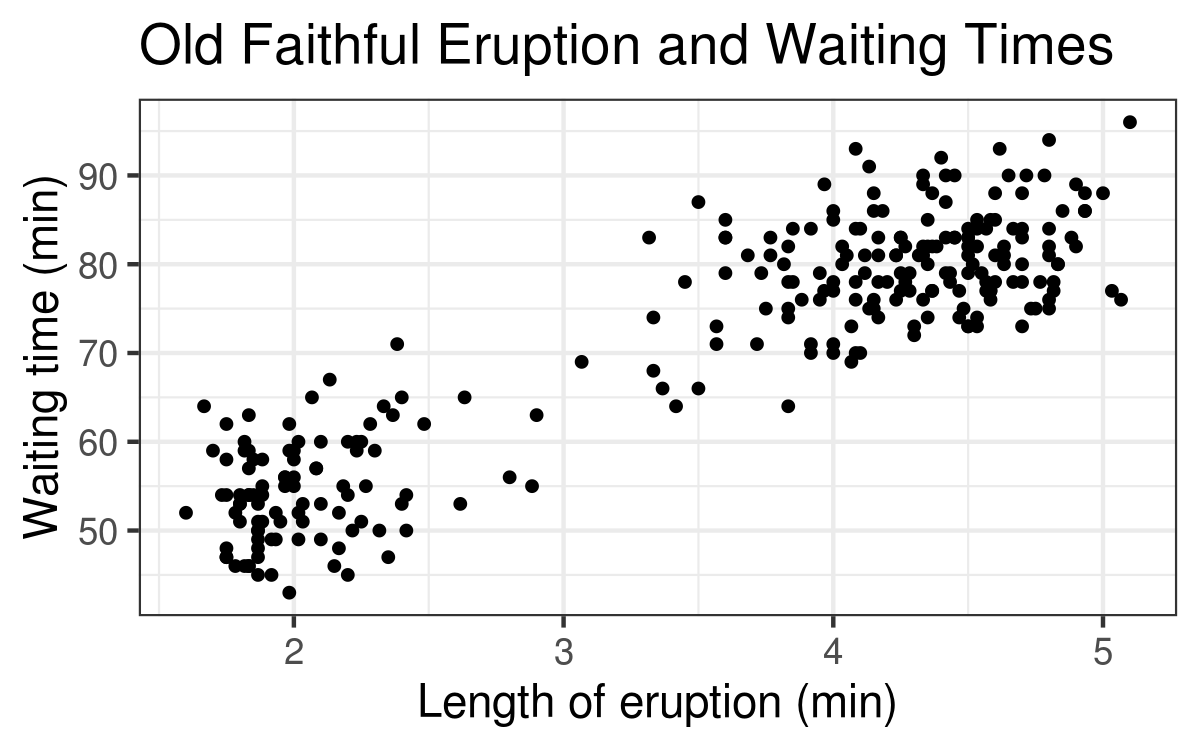
\includegraphics[width=4in]{images/group04_Q4_a}
\par}


\bigskip
\bt{There does seem to be a relationship between length of eruption and waiting time for next eruption.}



\newpage
\item[(b)] The data set ``hair\_eye.csv" contains the hair and eye color of 592 statistics students. The math department would like to know what is the most common eye color. What is the least common eye color?\\
\bigskip
\bt{Any graph that displays counts of categorical data could be used, such as pie charts or bar graphs. However, since we want to know the most and least common eye colors, a Pareto chart would be best. }
\bigskip

{\centering
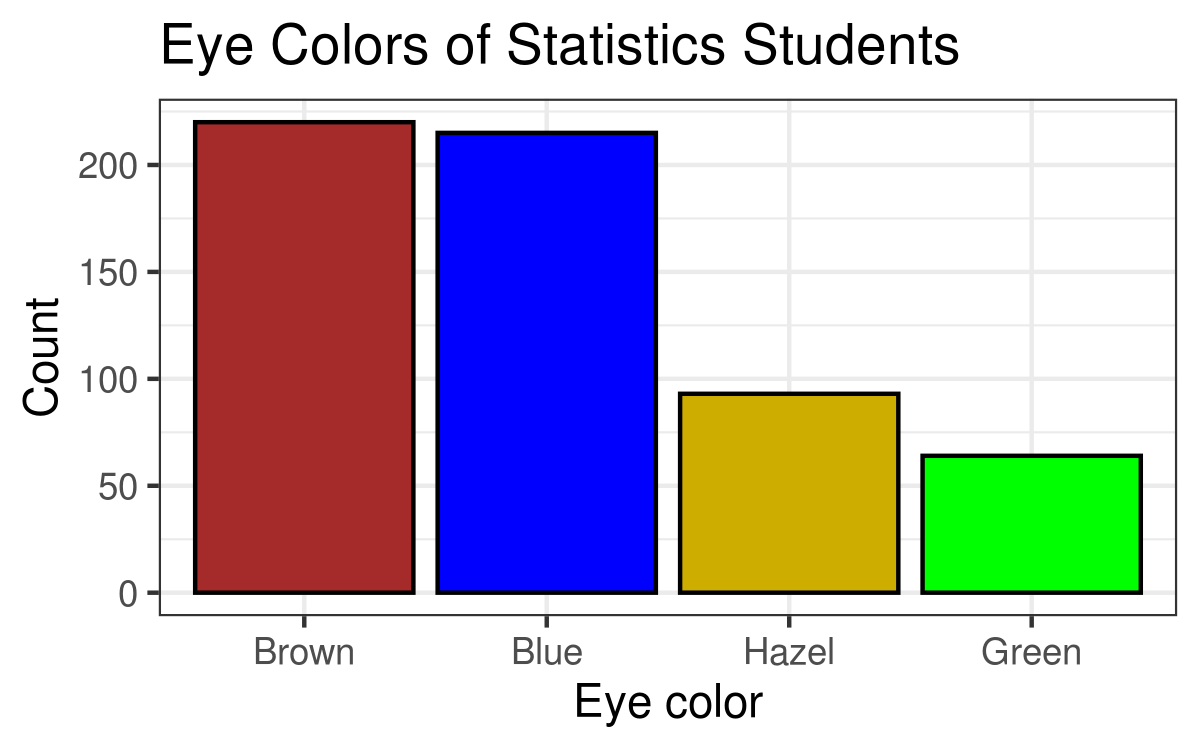
\includegraphics[width=4in]{images/group04_Q4_b}
\par}

\bigskip
\bt{The most common eye color is brown and the least common is green.}

\vspace{.25in}
\end{itemize}


\end{flushleft}
\end{document}